\documentclass{article}

\usepackage{titlesec}
\titlespacing*{\section}{0pt}{0.1em}{0.1em}
\titlespacing*{\subsection}{0pt}{0.1em}{0.1em}

\newcommand{\tabitem}{~~\llap{\textbullet}~~}

\usepackage{float}

\usepackage[a4paper, margin=1in]{geometry}
\usepackage[toc,page]{appendix}
\usepackage{graphicx}
\usepackage{adelaideuniTitle}
\usepackage{parskip}
\usepackage{graphicx}
\usepackage{amsmath}

\begin{document}

\supervisor{Qinfeng Shi and Dong Gong}
\project{Progress Report}
\author{Miguel Martin}
\title{Generating Videos From Text}

%
%
% TODO, tomorrow:
% in the monring:
% 1. background
% 2. references
% 3. review of literature 
%
% in afternoon:
% 1. progress
% 2. next semester
% 3. Intro + conclusion
%
% at night:
% 1. references
% 2. proof read
% 3. submit
%
%



\maketitle
\tableofcontents
\newpage

\section{Introduction} 

This report will cover my progress over the semester for my project. It will include necessary background information to understand
the progress I have made. 

\section{Background}

This section describes the surrounding material regarding the problem I am
researching. These subjects were researched in order to understand the state of Machine Learning related to my research topic to aid the implementation,
experimentation and possible advancements that could be made.

\subsection{Generative Modelling}

Generative modelling can be seen as an unsupervised learning task, where we are given a set of data and we are
tasked to generate more examples of the data from the same underlying distribution of where the data came from. For example, given some images of birds, generate another bird (but is not the same as the birds given). This can be viewed as learning the distribution of data via maximum likelihood (the distribution we learn
maximises the probability of our given samples). It is not required to learn generative models via maximum likelihood, but most can be viewed in this way, including GANs which do not explicitly model the problem
with an explicit density function \cite{goodfellow_nips_2016}.

\subsection{Generative Adversarial Networks (GANs)}

Generative Adversarial Networks (GANs) were introduced by Ian Goodfellow and others
in 2014 \cite{goodfellow_generative_2014}. They structure learning the
generative task as a two player game, where you have a generator and
discriminator competing against each other. The discriminator's job is to
determine if a given sample is generated (fake) or real. The generator produces
fake/generated samples with the goal of fooling the discriminator. In the
context of GANs, both the generator and discriminator are neural networks. In
general the term \textit{adversarial learning} is used when referring to this
methodology of learning, i.e. where an adversary aids the learning process.

Typically the generator network learns to produce data from some latent
vector. This vector can be described as some random sample from some known
distribution, e.g. the normal distribution. Thus the generator can be viewed as a mapping from some known distribution to some unknown distribution. My
interpretation of this is, you can interpret the latent variable(s) as necessary
(unknown) information required to generate the sample. 

In the case of conditional GANs, we simply make this latent variable be the concatenation of
the information we are conditioning on and the previously described latent
variable. We make the discriminator determine if the pairing of the sample and conditioning information
belong together. Thus, conditional GANs also require to make the discriminator output on a mismatch of a real sample and incorrect conditioning information with the goal to output. In the context of our problem it would be a pair of real video and incorrectly associated text \cite{li_video_2017,pan_create_2018}.

The training process of GANs can be simply described. Stochastic Gradient
Descent (SGD) or some variant (Adam \cite{kingma_adam:_2014} is a good choice) 
is performed simultaneously for both the generator and discriminator networks. For each mini-batch, we: 

\begin{enumerate}
    \item Generate a latent variable for each sample and let the generator
        produce the associated samples
    \item Let the discriminator predict whether it thinks the generated
        and real samples are real or fake. Assuming the discriminator
        outputs 0 or 1 (or anything in between) we can assign the loss of the
        discriminator as binary cross-entropy as is usually done with GANs \cite{goodfellow_nips_2016}.
    \item After updating the discriminator with SGD, we can again see what the discriminator predicts 
          for the fake samples. This time, we will update the generator's weights to make the discriminator think
          that these samples are real, again by optimising binary cross-entropy loss.
\end{enumerate}

During the training process itself, it is quite different to typical
optimisation problems, where we aim to minimise our loss. We can still view GANs 
as a form of supervised learning \cite{goodfellow_nips_2016}, but instead, we
care more about the discriminator and generator as a whole. We hope
both players of the game are approximately equals such that they can
continue improve over time. Ideally we want to reach/converge to a Nash equilibrium \cite{goodfellow_nips_2016}.

Thus during the training process we hope the discriminator nor the generator
over-powers each other by too large of a margin. It is typical when training GANs to modify the hyper-parameters
of the learning algorithm in order for this to not be the case, e.g. simplify/increase complexity of the discriminator
if the discriminator's loss converges to 0 or diverges, modify the learning rates of the generator/discriminator, etc. 

\subsubsection{DCGAN}

DCGAN stands for deep convolutional GAN \cite{radford_unsupervised_2015}. Most GANs are based on the DCGAN architecture \cite{goodfellow_nips_2016}. The architecture is composed of:

\begin{enumerate} 
    \item Batch normalization in performed in most (if not all) layers of both the generator and discriminator except for the last layer
    \item Each network is purely convolutional, borrowing from \cite{springenberg_striving_2014}
    \item Adam optimizer is utilized
\end{enumerate}

\subsubsection{WGAN and WGAN-GP}

In the typical GAN setup the generator can be seen as optimising the Jensen Shannon divergence between 
the real distribution of data and the learnt (implicit) distribution of data. This is the main reason for why
it is believed GANs have such great performance, as typical Maximum Likelihood models learn by minimising 
KL-divergence \cite{goodfellow_nips_2016}.

The WGAN paper hypothesises (and empirically proves) some problems with minimising JS-divergence and 
instead advocates minimising Wasserstein-1 (Earth-Mover) distance \cite{arjovsky_wasserstein_2017}. Specifically 
they demonstrate with a toy example, that JS-divergence (and KL-divergence) does not provide a smooth differential 
function, which is useful when performing gradient descent \cite{weng_gan_nodate}. Earth-Mover distance between two 
probability distributions can be viewed as the amount of dirt required to move, with minimum cost (i.e. with the least amount of work required), in order to transform one distribution to the other \cite{arjovsky_wasserstein_2017}. Earth-Mover 
distance has some nice proprieties, such as symmetry

There is one major constraint with WGAN, and that is the weights of the network must be clipped between a range of values $[-c, c]$ (for some hyper-parameter $c$), as it 
must be a 1-Lipschtiz function \cite{arjovsky_wasserstein_2017}. WGAN-GP (gradient penalty) suggests a method of not requiring this constraint, by penalising the model
if the norm of the gradient is too far away from the value 1 (how big this penalty is adjustable via a hyper-parameter). They obtain higher quality
images than the original WGAN \cite{gulrajani_improved_2017}.

\section{Review of Literature}

There are four main papers covering the task of video generation. All of which were reviewed. Following will be a brief summary of all four papers.

\subsection{Video Generation From Text}

They model the problem with generative models, specifically a hybrid approach with a conditional Variational Auto Encoder (c-VAE) and a DCGAN with 3D de-convolutional layers in the generator and 3D convolutional layers in the discriminator \cite{li_video_2017}. They propose the use of a gist which is predicted by the conditional Variational Auto-Encoder, conditioned on the first frame of the video during the training process (and unconditioned during evaluation). This gist aims to simultaneously
capture the layout/structure of objects within the video and the background colour/general aesthetics of the video \cite{li_video_2017}. They also utilise the WGAN algorithm for learning \cite{arjovsky_wasserstein_2017}.

Text is encoded with an RNN, specifically a bi-directional LSTM. Then their generator network simply takes in the concatenation of the text feature they predict alongside their gist. They introduce what they call `Text2Filter' which is simply a convolutional layer with the input text feature vector concatenated and copied along the channels of the gist image, as they noticed that without this the model give too much emphasis to the text or gist image \cite{li_video_2017}. The discriminator also
uses `Text2Filter', but with the input video instead of the gist.

The data they use is simple sentences describing an action to short video clips from the Kinetics Human Action Video Dataset \cite{kay_kinetics_2017}, with video resized to 64x64 and at a length of 32 frames. Finally, they conclude that their approach out-performs other simpler approaches, namely their model without the inclusion of the `gist' and Text2Filter (both combinations of the two). As videos are associated with actions, they perform similar akin to an Inception score for quantitative
comparisons, by having a separate model predict the associated action for an output video.

\subsection{To Create What You Tell: Generating Videos from Captions}

`To Create What You Tell` (TCWYT) \cite{pan_create_2018} and `Video Generating from Text' \cite{li_video_2017} both have many similarities. They both utilise GANs, but TCWYT does not utilise
a VAE or predict a `gist' or background prior to generating the video. Instead, they propose three additional discriminators:

\begin{enumerate}
    \item A discriminator that determines if video and sentence pairings are correlated
    \item A discriminator that determines if individual and sentence pairings are correlated.\\
        From a theoretical perspective this is equivalent to the above, but they notice that from an empirical perspective 
        the model out-performs without it.
    \item A discriminator to determine if motion (temporal coherence) is correctly associated with the given sentence.\\
        Motion is simply described as the difference between two frame. Specifically the difference between the features of each frame (as predicted by the above model). They propose
        an alternative to this and that is to minimise the difference of two frames via L2 norm, but they hypothesis and show empirically that adversarially learning this is significantly better.
\end{enumerate}

To give the discriminators the input of a 3D or 2D matrix concatenated with text for conditioning purposes, they also perform something equivalent to `Text2Filter' as described in the previous paper \cite{li_video_2017,pan_create_2018}. The `Text2Filter' only after to the text vector being transformed with a fully connected layout first.

The data they use is YouTube cooking clips from the Microsoft Research Video Description Corpus (MRVDC) dataset \cite{noauthor_microsoft_nodate}. The quantitative measure they utilise is what is referred to as a Generative Adversarial Metric (GAM). This metric puts two generative adversarial models against each other in battle. It utilises the ratio of correct classifications from a test distribution, and also compares the number of times a discriminator is fooled by the opponents generator. The winner is defined by a simple heuristic which favours the ability to fool the opponent assuming the classification accuracy is approximately the same. They produce reasonable results, one might argue slightly better than the previous paper.

\subsection{Imagine This! Scripts to Compositions to Videos}

This paper introduces an iterative algorithm to produce videos, with a model referred to as \textbf{C}omposition, \textbf{R}etrieval \textbf{a}nd \textbf{F}usion Ne\textbf{t}work (CRAFT) \cite{gupta_imagine_2018}. This model
aims to jointly learn the layout of characters and objects alongside the appearance of the objects. However, unlike the previous two, the appearance of the model is modelled as an image retrieval task. They experiment
with producing image pixels but notice very blurry results. Due to this, not much emphasis on this paper was performed. As one can guess, this approach is very restricted in terms of the data utilised, and as such
they limit themselves to generating the Flinstones cartoon.

They claim that predicting visual information directly in high dimensional space is inadequate to address the following challenges: \cite{gupta_imagine_2018}. These are are similar to 
those described in my proposal:

\begin{enumerate}
    \item Entity Recall
        \begin{itemize}
            \item Retrieve relevant characters and objects
            \item Retrieve relevant 
        \end{itemize}
    \item Layout feasibility: plausible locations and sizes of entities
    \item Appearance Fidelity: appearance of entities must respect the scene description
    \item Interaction Consistency. Appearance of entities must be consistent relative to each other given context (description of the scene or implied behaviour/interactions, 
        such as facing each other whilst talking)
    \item Language Understanding: Translate a natural language description into a plausible visual instantiation
\end{enumerate}

Their algorithm at a very high level works as follows, they iteratively construct their video and feed it back into their algorithm. They have
two models a `Layout Composer' (outputs location and scale given the partially constructed video and noun/entity) and 
an entity retriever (performs k-NN retrieval given partially constructed video and noun). During the training (and evaluation) process, we perform the iterative steps:

\begin{enumerate}
    \item For the entire sentence, retrieve the correctly associated background
    \item For each entity (noun) in the text, they perform the two steps:
        \begin{enumerate}
            \item Create a new empty frame, based off the previous frame
            \item Predict the location and scale of the entity with the layout model
            \item Retrieve the associated entity with the entity retriever
            \item Combine with the previous frame, set this frame as the new frame to base future frames off of. Combination is simply done by placing the entity over the associated position.
        \end{enumerate}
\end{enumerate}

They train the system in an iterative process. Text is fed through a bi-directional LSTM. It is not very clear from the text on how they know when to stop iterating or how they generate more frames than entities. It should be noted
that they predict the location and scale by explicitly modelling a distribution through a Multi-Layer Perceptron.

\section{Progress}

The progress I have made throughout the semester is composed of theory/research (as stated in previous sections) and the implementation of a baseline generative model. My first
initial steps from a practical perspective included learning the framework
PyTorch \cite{paszke_automatic_2017}, implementing DCGAN \cite{radford_unsupervised_2015} for generating images, extending this to generate images from text, and then 
finally implementing the paper `To Create What You Tell' \cite{pan_create_2018}. The paper was implemented as no implementation was 
publicly available, to solidifying my understanding and as I believed it to have the best results for video generation from text. There are some differences in my implementation of their paper, most notably:

\begin{enumerate}
    \item Added L1 reconstruction loss, similar to that of \cite{li_video_2017}, but I noticed that it did contribute to mode-collapse with respect to the datasets I used. 
    \item Picking the correct video and wrong sentence pair was done by choosing a random permutation from mini-batch, and thus there may be situations where this pair is actually associated together (it was ensured
        that the identity permutation was not generated). This
        would only be probable for the toy dataset, which may be the main contributing factor for the artefacts.
    \item I am not using a bi-directional LSTM; this difference will be changed relatively soon.
\end{enumerate}

Pre-training of the sentence RNN encoder \cite{dai_semi-supervised_2015} as suggested in \cite{pan_create_2018}
was also implemented. During this pre-training process, teacher forcing was only
utilised with probability $0.2$. The sentence encoder was composed of a simple LSTM (uni-directional), and 
word embedding was performed prior to feeding the sequence of words to the recurrent model. Words were embedded to 
vectors of dimensionality 128, the LSTM hidden states had dimensionality 256 and due to this the final sentence was embedded to a vector
of dimensionality 256.

Two datasets were utilised for the experimental setup, both stemming from the experimental setup as described in \cite{pan_create_2018}. The first was a toy dataset, composed of synthetically produced videos where one MNIST \cite{yann_mnist_nodate} 
digit would move across the screen; code was written in order to generate this dataset. The second dataset was cooking video clips from the
Microsoft Research Video Description Corpus (MRVDC) \cite{noauthor_microsoft_nodate} dataset 
as done in \cite{pan_create_2018}, however sentences longer than 60 characters were also filtered out.

\subsection{Toy Dataset}

A training dataset of 40,000 video clips was generated. Every combination of
each possible sentence describing a digit in motion was available within this training
set. The sentences were of the form 'the digit [0-9] is moving \{{\{up,down\},
\{left,right\}\} \{and,to\} \{{\{down,up\}, \{right,left\}\}'. That is, a digit
could move left to right (or vise-versa) or up and down (or vise versa), i.e. 4
unique directions. Clips were generated to be 32 frames long (at 30 frames per
second), with each frame consisting 64x64 pixels, with each digit
resized to 28x28 pixels. The digits would move back and forth between
two points either horizontally (if left/right) or vertically (if
up/down), with the initial direction specified in the text. The two
positions the digits would moving between were randomly generated, with
random speed associated with them.

Doing some quick math shows there are 40 possible combinations of the sentences
provided. With 6,000 digits per class in MNIST (in the training set)
\cite{yann_mnist_nodate}, there are 240,000 possible sentences associated with a
unique hand-written digit. 

Looking at the produced videos from a trained generative model, there are some notable issues, namely:

\begin{enumerate}
    \item Occasional training artifacts in some iterations of the training
        process for some associated frames. I believe this is due to my
        activation functions obtaining a negative slope, but since LeakyReLU
        \cite{xu_empirical_2015} was utilised this issue resolved itself with further
        iterations. This can be seen in Figure 2.
    \item Mode collapse as shown with Figure 3. This is likely due to there
        only being 36 possible combinations of the sentences, and thus it was
        likely learnt to simply generate from the sentence itself (i.e. the
        latent variable was ignored). This hypothesis is supported with the other dataset I tested with.
    \item Issues in the produced videos, i.e. moving in the wrong direction, morphing of digits. This can be seen in Figure 4. Likely due to the discriminators not performing correct classification (i.e. confusion with some digits). It is not clear how to resolve this issue.
\end{enumerate}

\begin{figure}[H] \label{fig:abc2}
    \centering
    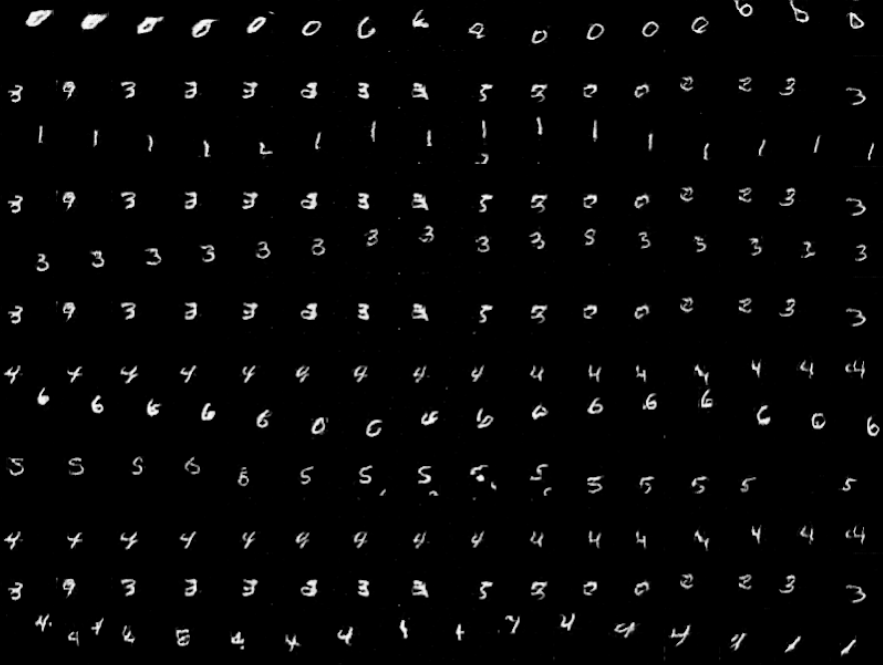
\includegraphics[width=0.45\linewidth]{imgs/mnist/fake_mnist.png}
    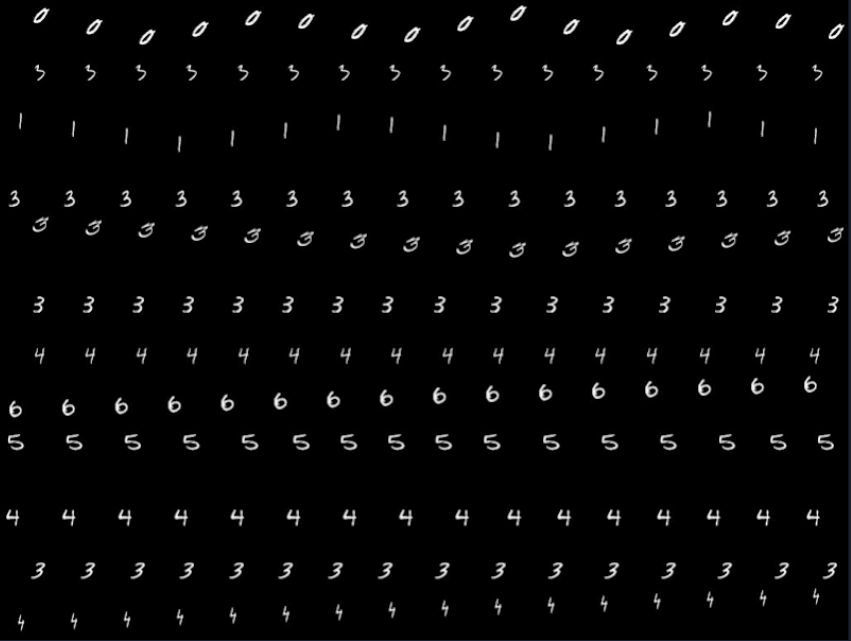
\includegraphics[width=0.45\linewidth]{imgs/mnist/true_mnist.png}
    \caption{Fake samples (left) vs. real samples (right) on MNIST toy dataset}
\end{figure}

\begin{figure}[H] \label{fig:abc}
    \centering
    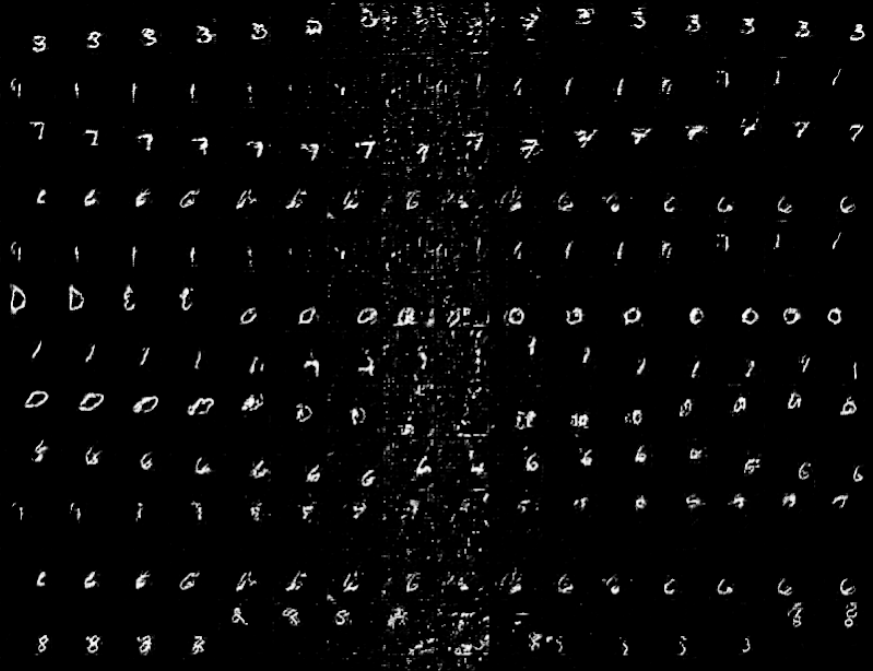
\includegraphics[width=0.8\linewidth]{imgs/mnist/mnist_artifacts.png}
    \caption{Occasional artifacts from training}
\end{figure}

\begin{figure}[H] \label{fig:modecollapse}
    \centering
    
\includegraphics[width=0.8\linewidth]{imgs/mnist/mode_collapse.png}\\
    
\includegraphics[width=0.8\linewidth]{imgs/mnist/mode_collapse2.png}
    
\includegraphics[width=0.8\linewidth]{imgs/mnist/mode_collapse3.png}
    \caption{Three generated samples with the same sentence but different latent variables (evidence of mode collapse)}
\end{figure}

\begin{figure}[H]
    \centering
    
\includegraphics[width=0.8\linewidth]{imgs/mnist/minst_9_true.png}\\
    
\includegraphics[width=0.8\linewidth]{imgs/mnist/minst_fake_9.png}
    \caption{Video for the text `the digit 9 is moving down and up' (real is top, generated is bottom)}
\end{figure}

\subsection{MRVDC}

This dataset was filtered out to have simple cooking clips, as shown in
Figure 7. This is performed in \cite{pan_create_2018}, as these clips are
relatively simple since they mostly are composed of close-ups of chopping
vegetables, boiling a pot of water/soup, etc. Sentences of longer than 60
characters were also removed, due to these sentences being very verbose. There were multiple sentences belonging
to the same video clips. There were 387 video clips in total, but they were
randomly split into a training and validation set with a split ratio of 80:20.
This left 308 videos in the training set and 79 in the validation set.
Splitting was done to ensure there were sentences that were not seen by the
model. The training set was the only set used for training purposes, including for the sentence encoder.

Poor video quality seems to be an issue, some produced videos are completely
non-sensical as shown in Figure 6. However, some videos generated do show
some promise, as shown in Figure 5. The poor quality and outliers may be due
to lack of quantity of data and diversity. No outliers were demonstrated in
\cite{pan_create_2018}, which leaves me to believe that there might have been
heavy cherry picking. Mode collapse is definitely not a large issue with this dataset, but to some degree it does 
crop up to some degree.

\begin{figure}[H]
    \centering
    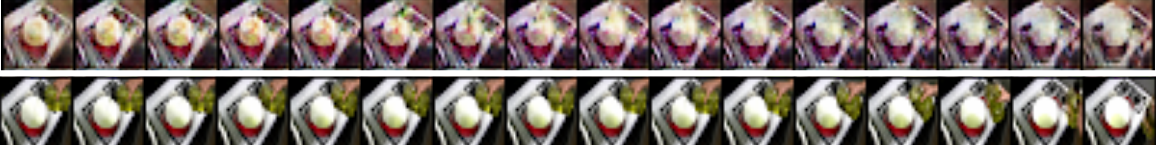
\includegraphics[width=0.8\linewidth]{imgs/mrvdc/good_1.png}\\
    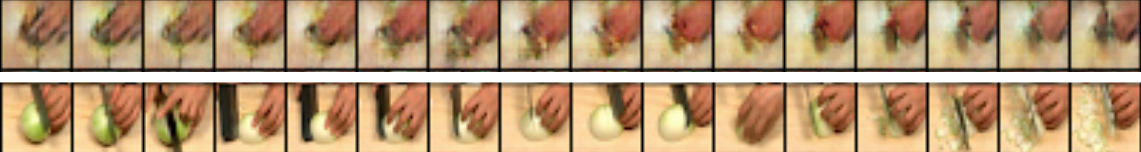
\includegraphics[width=0.8\linewidth]{imgs/mrvdc/good_2.png}
    \caption{Good visual results from two different videos (sampled from the training set).}
\end{figure}

\begin{figure}[H]
    \centering
    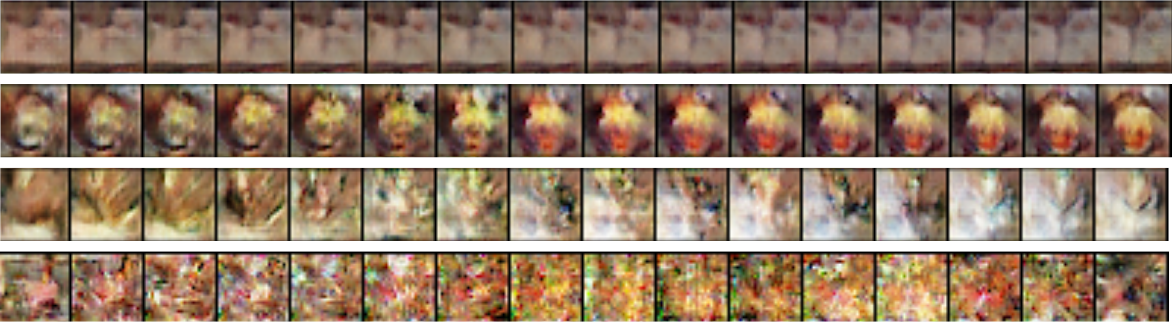
\includegraphics[width=0.8\linewidth]{imgs/mrvdc/bad_quality.png}
    \caption{Bad quality videos sampled from the training.}
\end{figure}

\begin{figure}[H]
    \centering
    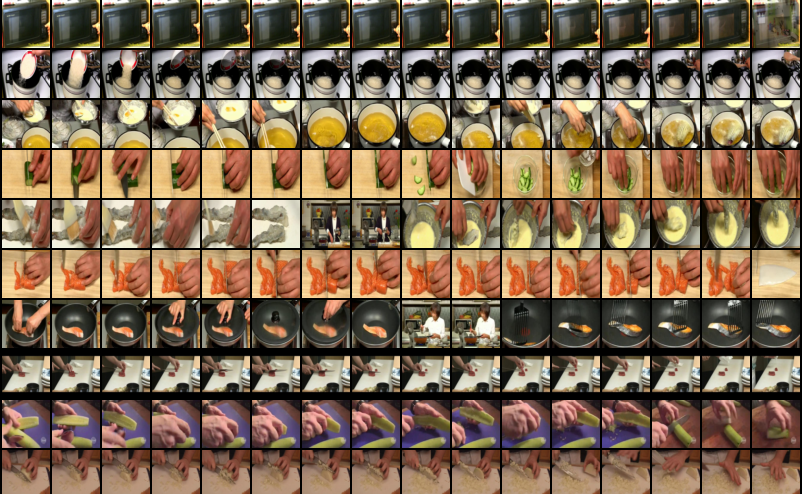
\includegraphics[width=0.8\linewidth]{imgs/mrvdc/real_samples.png}
    \caption{Some example real videos from the dataset}
\end{figure}

\begin{figure}[H]
    \centering
    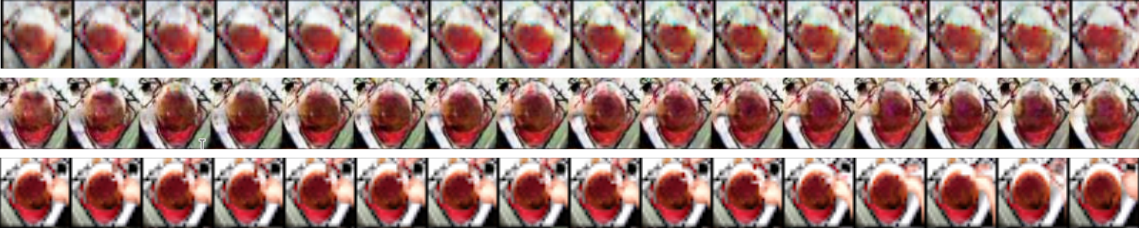
\includegraphics[width=0.8\linewidth]{imgs/mrvdc/compare.png}
    \caption{A comparison from the original paper (top), with my results (middle) and a real sample (bottom). }
\end{figure}

\begin{figure}[H]
    \centering
    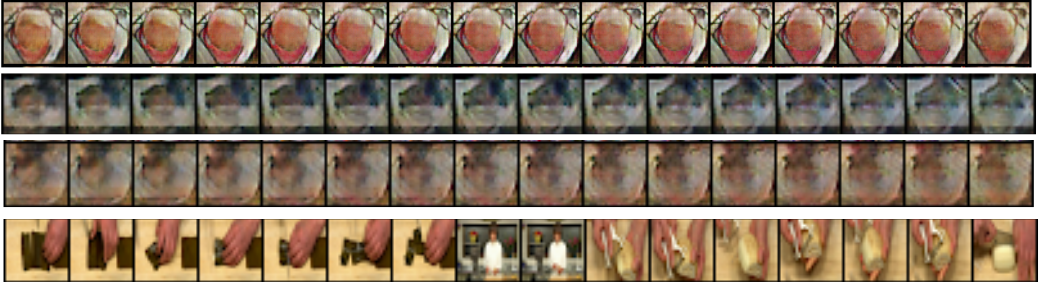
\includegraphics[width=0.8\linewidth]{imgs/mrvdc/test1.png}
    \caption{Three samples from the testing set with the ground truth on the bottom. For the sentence (tokenized): `$<$start$>$ a woman is saying about how to make vegetable tofu $<$unk$>$ $<$end$>$'}
\end{figure}

\begin{figure}[H]
    \centering
    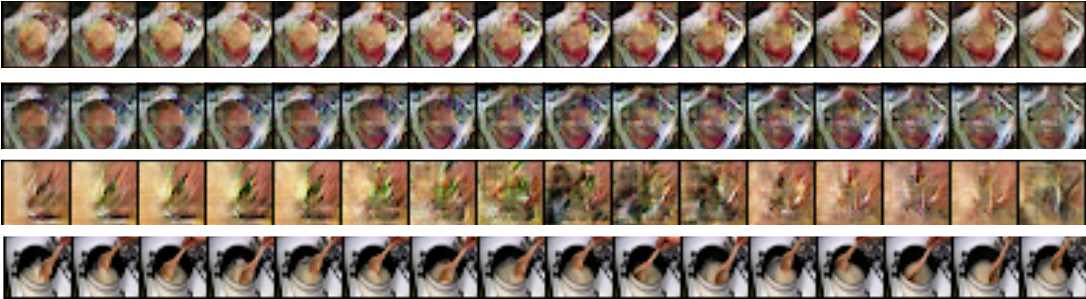
\includegraphics[width=0.8\linewidth]{imgs/mrvdc/test2.png}
    \caption{Three samples from the testing set with the ground truth on the bottom. For the sentence (tokenized): `$<$start$>$ the person is cooking $<$end$>$'}
\end{figure}

\section{Next Semester}

The main goal for next semester is to produce better results than what has currently 
been achieved, with respect to visual quality, length, and diversity. I hypothesise that this
can be achieved in three main ways: 

\begin{enumerate}
    \item Utilisation of modern techniques. This might include: 
        \begin{itemize}
            \item Using invertible networks to reduce memory consumption requirements, perhaps with Recurrent Neural Networks as proposed in \cite{mackay_reversible_2018}, as they 
                  note a 5 to 15 times memory reduction factor with the same results as their non-invertible counter-part. However, the notable caveat is the requirement
                  to make a network invertible may require more memory for an equivalent network; further research and understanding is required.
            \item Using modern advancements with respect to the specific generative model, e.g. for GANs there are numerous additional heuristics to aid, which 
                has been described in the background section (see sections under `Background' labelled: GAN, WGAN, WGAN-GP, and StackGAN and variants)
        \end{itemize}
    \item Utilisation of more data both in terms of quantity and diversity.\\
         It is well known that deep networks need large quantities of data. Perhaps with large amounts of data, video quality improves.
    \item Different structuring of the problem. This ties in with my first hypothesis, but for example this might include
        \begin{itemize}
            \item Solving multiple problems at once, which may aid in the process of the original problem
            \item Utilising domain knowledge, e.g. similar to that of using scene graphs \cite{johnson_image_2018} as discussed in my proposal report
        \end{itemize}
\end{enumerate}

My plan for next semester and the Summer Holidays, is described in detail with
an associate set of goals, purpose and deliverables which will be performed at
the end of the month. It is hard to predict future events, due to this, the
feasibility of each month's deliverables will be evaluated in each meeting with
my supervisors. If they are classified as infeasible, some adjustments to the
plan may be performed. These adjustments may involve: focus on a particular
approach, a constraint on the types of videos generated (e.g. only cartoons),
further simplification of the problem, utilisation of domain knowledge (notably
scene graphs \cite{johnson_image_2018}), etc.

Throughout each month, fundamental theory will be revised and learnt in order to
solidify and enhance my understanding of the generative problem.

\subsection{November}

\subsubsection{Goals and Purpose}

To evaluate if advancements in GANs play a large impact on the quality of videos that can be produced, and separately to see if larger and more diverse datasets also play a big impact on the quality of videos. To do this, I will experiment with:

\begin{enumerate}
    \item GAN advancements
    \item Larger quantities of data
    \item More diversity in videos (separate and combined with the above)
\end{enumerate}

\subsubsection{Deliverables}

\begin{enumerate}
    \item Implementation of WGAN and WGAN-GP
    \item Use of bi-directional LSTMs
    \item Three new datasets to use for further experimentation, aimed to cover: low/high diversity and low/high quantity of data
\end{enumerate}

\subsection{December}

\subsubsection{Goals and Purpose}

To evaluate if higher dimensionality negatively impacts the performance of the models. To do this, I will experiment with:

\begin{enumerate}
    \item Longer and shorter videos
    \item Higher resolution videos
    \item Implementation of StackGAN++ \cite{zhang_stackgan++:_2017}, perhaps on small video lengths in memory is a problem
    \item See if AttnGAN \cite{xu_attngan:_2017} is possible to implement for this problem
\end{enumerate}

\subsubsection{Deliverables}

\begin{enumerate}
    \item Implementation of StackGAN++ \cite{zhang_stackgan++:_2017}
    \item Evaluation of how much time negatively impacts the visual quality and diversity of produced videos
    \item Determine the limit on the length and resolution of the videos we can generate, both from theoretical and practical points of view
\end{enumerate}

\subsection{January}

\subsubsection{Goals and Purpose}

The goal of this month is to evaluate if there are alternative generative models or modifications to existing models to produce high quality videos with reasonable lengths of time (at least 2 seconds long).

\begin{enumerate}
    \item Determine if a recurrent generative model is possible to create to remove time constraints and
          reduce the number of parameters required
    \item See if reversible recurrent models can be applied to the above, as they can reduce
        the number of parameters required by a factor of 10-15 fold with the same performance as their non-invertible counter-part \cite{mackay_reversible_2018}
    \item Experiment/learn further about invertible generative models, such as GLOW \cite{kingma_glow:_2018}, to see if they can be applied and perform well on videos
\end{enumerate}

\subsubsection{Deliverables}

\begin{enumerate}
    \item An analysis if further development of any of these approaches should be performed, by evaluating and comparing them to the current state of work
\end{enumerate}

\subsection{February}

\subsubsection{Goals and Purpose}

Formalise and implement the experimental setup and quantitative analysis of models, such as an Inception score. Ideally the quantitative analysis should cover all possible
dimensions of what we care about, such as video quality, diversity, motion, correspondence to the text, visual and layout consistency over time, etc. (described in much detail in my proposal).

\subsubsection{Deliverables}

\begin{enumerate}
    \item A formal experimental methodology, including: 
        \begin{itemize}
            \item A dataset or set of datasets to evaluate the performance of different dimensions of the problem
            \item A way to quantitatively compare models, such as an Inception score as done in \cite{zhang_stackgan++:_2017} or Generative Adversarial Metric (GAM) as done in \cite{pan_create_2018}
        \end{itemize}
    \item An implementation of the quantitative analysis
\end{enumerate}

\subsection{March}

\subsubsection{Goals and Purpose}

This month is dedicated to experimentation and finalisation of the current models, with the experimental setup developed in the previous month.

\subsubsection{Deliverables}

\begin{enumerate}
    \item A comparison between each model developed throughout the semester
    \item Improvements over existing work
\end{enumerate}

\subsection{April}

\subsubsection{Goals and Purpose}

This month is dedicated to the same as the previous month, with the addition of the starting a draft of my thesis.

\subsubsection{Deliverables}

A draft of my thesis will be written by the end of this month.

\subsection{June (until week 13)}

\subsubsection{Goals and Purpose}

By this deadline, my thesis and presentation will be written.

\subsubsection{Deliverables}

Thesis and presentation.

\section{Conclusion}

This report covered the background information necessary to understand the current progress of my project. It touched on the results of my paper, which was the implementation of \cite{pan_create_2018}. The Summer Holidays and next semester have been planned out in terms of what I am wanting to achieve on a month-by-month basis. The main goal for next semester is to improve upon the current results, experiment further with adversarial models and alternative generative models. It is my goal to produce good quality videos will be produced by the end of the semester, in terms of various dimensions I mentioned in my original proposal (such as considering motion, video quality, diversity, visual/layout consistency, etc.).

\newpage
\bibliography{ref}
\bibliographystyle{ieeetr}

\end{document}
